\documentclass[a4paper,oneside,12pt]{extreport}

\usepackage{mmap}
\usepackage[T2A]{fontenc}
\usepackage[utf8]{inputenc}
\usepackage[english,russian]{babel}


% Текст отчёта следует печатать, соблюдая следующие размеры полей:
% левое — 30 мм, правое — 15 мм, верхнее и нижнее — 20 мм.
\usepackage[left=20mm, right=15mm, top=15mm, bottom=15mm]{geometry}

% \setlength{\parindent}{1.25cm} % Абзацный отступ

\usepackage{setspace}
%\onehalfspacing % Полуторный интервал

\frenchspacing % Равномерные пробелы
\usepackage{indentfirst} % Красная строка

\usepackage{microtype}
\sloppy

\usepackage{titlesec}
\titlespacing*{\chapter}{0pt}{-30pt}{8pt}
\titlespacing*{\section}{\parindent}{*4}{*4}
\titlespacing*{\subsection}{\parindent}{*4}{*4}
\titleformat{\chapter}{\LARGE\bfseries}{\thechapter}{20pt}{\LARGE\bfseries}
\titleformat{\section}{\Large\bfseries}{\thesection}{40pt}{\Large\bfseries}

\usepackage{graphicx}
\usepackage{caption}

\usepackage[unicode,pdftex]{hyperref}
\hypersetup{hidelinks}

%% title begin
\usepackage{wrapfig}

\makeatletter
	\def\vhrulefill#1{\leavevmode\leaders\hrule\@height#1\hfill \kern\z@}
\makeatother
%% title end

%% begin code
\usepackage{listings}
\usepackage{xcolor}

\lstset{
	basicstyle=\footnotesize\ttfamily,
	breakatwhitespace=true,
	breaklines=true,
	commentstyle=\color{gray},
	frame=single,
	keywordstyle=\color{blue},
	stringstyle=\color{red},
	tabsize=8
}

\lstdefinestyle{lispinline}{
	frame=none,
	language=Lisp
}

\newcommand{\code}[1]{\texttt{#1}}
%% end code

%% begin theorem
\usepackage{amsthm}

\makeatletter
\newtheoremstyle{indented}
	{}% measure of space to leave above the theorem
	{}% measure of space to leave below the theorem
	{}% name of font to use in the body of the theorem
	{\parindent}% measure of space to indent
	{\bfseries}% name of head font
	{.}% punctuation between head and body
	{ }% space after theorem head; " " = normal interword space
	{}% header specification (empty for default)
\makeatother

\theoremstyle{indented}

\newtheorem{definition}{Определение}[section]
\newtheorem{example}{Пример}[section]
\newtheorem{theorem}{Теорема}[section]
\newtheorem{task}{Задание}

\makeatletter
\DeclareRobustCommand\bfseriesitshape{%
	\not@math@alphabet\itshapebfseries\relax
	\fontseries\bfdefault
	\fontshape\itdefault
	\selectfont
}
\makeatother

\DeclareTextFontCommand{\textbfit}{\bfseriesitshape}
\DeclareTextFontCommand{\define}{\bfseriesitshape}
%% end theorem

%% begin columns
\usepackage{etoolbox,refcount}
\usepackage{multicol}

\newcounter{countitems}
\newcounter{nextitemizecount}
\newcommand{\setupcountitems}{%
	\stepcounter{nextitemizecount}%
	\setcounter{countitems}{0}%
	\preto\item{\stepcounter{countitems}}%
}
\makeatletter
\newcommand{\computecountitems}{%
	\edef\@currentlabel{\number\c@countitems}%
	\label{countitems@\number\numexpr\value{nextitemizecount}-1\relax}%
}
\newcommand{\nextitemizecount}{%
	\getrefnumber{countitems@\number\c@nextitemizecount}%
}
\newcommand{\previtemizecount}{%
	\getrefnumber{countitems@\number\numexpr\value{nextitemizecount}-1\relax}%
}
\makeatother
\newenvironment{AutoMultiColItemize}{%
	\ifnumcomp{\nextitemizecount}{>}{3}{\begin{multicols}{2}}{}%
		\setupcountitems\begin{itemize}}%
		{\end{itemize}%
		\unskip\computecountitems\ifnumcomp{\previtemizecount}{>}{3}{\end{multicols}}{}}
\makeatother
\newenvironment{AutoMultiColEnumerate}{%
	\ifnumcomp{\nextitemizecount}{>}{3}{\begin{multicols}{2}}{}%
		\setupcountitems\begin{enumerate}}%
		{\end{enumerate}%
		\unskip\computecountitems\ifnumcomp{\previtemizecount}{>}{3}{\end{multicols}}{}}
%% end columns



\begin{document}

\begin{titlepage}
	{\large % 14pt instead of 12pt
	\onehalfspacing
	\centering

	\begin{wrapfigure}[7]{l}{0.14\linewidth}
		\vspace{3mm}
		\hspace{-10mm}
		
\includegraphics[width=\linewidth]{img/b_logo}
		% \includegraphics[width=0.93\linewidth]{inc/img/bmstu-logo}
	\end{wrapfigure}
	{\singlespacing \footnotesize \bfseries Министерство науки и высшего образования Российской Федерации\\Федеральное государственное бюджетное образовательное учреждение\\высшего образования\\<<Московский государственный технический университет\\имени Н.~Э.~Баумана\\ (национальный исследовательский университет)>>\\(МГТУ им. Н.~Э.~Баумана)\\}

	\vspace{-2.2mm}
	\vhrulefill{0.9mm}\\
	\vspace{-7.5mm}
	\vhrulefill{0.2mm}\\
	\vspace{2mm}

	{\doublespacing \small \raggedright ФАКУЛЬТЕТ \hspace{5mm} \underline{«Информатика и системы управления»}\\
	КАФЕДРА \hspace{10mm} \underline{«Программное обеспечение ЭВМ и информационные технологии»}\\}

	\vspace{20mm}

	\begin{center}
		\noindent\begin{minipage}{1.2\textwidth}\centering
			\textbf{ОТЧЕТ ПО ЛАБОРАТОРНОЙ РАБОТЕ №18,19}\newline
			\textbf{По курсу: "Функциональное и Логическое программирование"}\newline\newline\newline
		\end{minipage}
	\end{center}

	\vspace{20mm}

	\noindent ~~Тема \underline{~~~~~~~~~~~~~~~~~~~~~~~~~~Рекурсия в прологе.~~~~~~~~~~~~~~~~~~~~~~~~~~~~~~~~~~~~~~~~~~~}\newline
	\noindent ~~Группа \underline{~~~~~~~~~~~~~~~~~~~~~~~~~~~~~~~~~~~ИУ7-63Б~~~~~~~~~~~~~~~~~~~~~~~~~~~~~~~~~~~~~~~~~~~~~~~~~}\newline
	\noindent ~~Студент \underline{~~~~~~~~~~~~~~~~~~~~~~~~~~~~Сукочева А.~~~~~~~~~~~~~~~~~~~~~~~~~~~~~~~~~~~~~~~~~~~~~~~~~~}\newline
	\noindent ~~Преподаватель \underline{~~~~~~~~~~~~~~~~~Толпинская Н.Б.~~~~~~~~~~~~~~~~~~~~~~~~~~~~~~~~~~~~~~~~~~~~~}\newline
	\noindent ~~Преподаватель \underline{~~~~~~~~~~~~~~~~~~Строганов Ю. В.~~~~~~~~~~~~~~~~~~~~~~~~~~~~~~~~~~~~~~~~~~~~}\newline


	\begin{center}
		\vfill
		Москва~---~\the\year
		~г.
	\end{center}
	}



\end{titlepage}

\setcounter{page}{2}

\section*{Практическая часть}

\begin{task}
    Напишите функцию, которая умножает на заданное число-аргумент все числа из заданного списка-аргумента, когда
	
    a) все элементы списка — числа,
    \begin{lstlisting}[language=Lisp]
(defun f (lst num)
    (cond ((null lst) ())
    (T (cons (* num (car lst)) (f (cdr lst) num))) ) )
\end{lstlisting}

    Пример использования:
    \begin{lstlisting}[language=Lisp]    
(f '(1 2 3 4) 5) ;; (5 10 15 20)
    \end{lstlisting}

    б) элементы списка — любые объекты.
    \begin{lstlisting}[language=Lisp]
(defun f (lst num)
    (cond ((null lst) ())
    ((symbolp (car lst)) (cons (car lst) (f (cdr lst) num)))
    ((listp (car lst)) (cons (f (car lst) num) (f (cdr lst) num)))
    (T (cons (* num (car lst)) (f (cdr lst) num))) ) )
    \end{lstlisting}

    Пример использования:
    \begin{lstlisting}[language=Lisp]    
(f '(1 2 (3 4 a) (b) T 7) 2) ;; (2 4 (6 8 A) (B) T 14)
    \end{lstlisting}
\end{task}

\begin{task}
    Напишите функцию, \code{select-between}, которая из списка-аргумента,
	содержащего только числа, выбирает только те, которые расположены между
    двумя указанными границами-аргументами и возвращает их в виде списка

    \begin{lstlisting}[language=Lisp]
(defun check-border (x a b)
    (and (>= x a) (<= x b)) )

(defun select-between (lst a b)
	(cond ((null lst) ())
	((symbolp (car lst)) (cons (car lst) (select-between (cdr lst) a b)))
	((listp (car lst)) (cons (select-between (car lst) a b) (select-between (cdr lst) a b)))
	((check-border (car lst) a b) (cons (car lst) (select-between (cdr lst) a b)))
	(T (select-between (cdr lst) a b))) )
    \end{lstlisting}

    Пример использования:
    \begin{lstlisting}[language=Lisp]    
(select-between '(1 2 (a b 3 4) T c 4 6 11 5) 2 7) ;; (2 (A B 3 4) T C 4 6 5)
    \end{lstlisting}
\end{task}

\begin{task}
    Что будет результатом (mapcar 'вектор '(570-40-8))

    mapcar примерняет свой первый аргумент поэлементно к своим аргументам.
    Т.е. первым аргументом должна быть функция. В нашем случае функции 'вектор' нет. 

    Результат: Error: ВЕКТОР is undefined.
\end{task}


\begin{task}
    Напишите функцию, которая уменьшает на 10 все числа из списка аргумента этой функции.

    \begin{lstlisting}[language=Lisp]
(defun f-func (lst)
    (mapcar (lambda (x) (- x 10)) lst))
    \end{lstlisting}

    \begin{lstlisting}[language=Lisp]
(defun f-rec (lst)
    (cond ((null lst) ())
    ((symbolp (car lst)) (cons (car lst) (f-rec (cdr lst))))
    ((listp (car lst)) (cons (f-rec (car lst)) (f-rec (cdr lst))))
    (T (cons (- (car lst) 10) (f-rec (cdr lst))))) )    
    \end{lstlisting}

    Пример использования:
    \begin{lstlisting}[language=Lisp]  
(f-func '(11 12 13 14 1))       ;; (1 2 3 4 -9)  
(f-rec '(11 12 13 14 1))        ;; (1 2 3 4 -9)
(f-rec '(11 12 (14 b 15) 16))   ;;(1 2 (4 B 5) 6)
    \end{lstlisting}
\end{task}

\begin{task}
    Написать функцию, которая возвращает первый аргумент
    списка-аргумента, который сам является непустым списком.

    \begin{lstlisting}[language=Lisp]
(defun f (lst)
	(cond ((null lst) NIL)
	((null (car lst)) NIL)
	(T (car lst))) )
    \end{lstlisting}

    Пример использования:
    \begin{lstlisting}[language=Lisp]    
(f '(Nil 1 2 3)) ;; NIL
(f '((1 2 3) 4 5 6)) ;; (1 2 3)
    \end{lstlisting}
\end{task}
    
\begin{task}
    Сумма числовых элементов смешанного структурированного списка
    \begin{lstlisting}[language=Lisp] 
(defun f-rec (lst num)
	(cond ((null lst) num)
	((symbolp (car lst)) (f-rec (cdr lst) num))
	((listp (car lst)) (+ (f-rec (car lst) 0) (f-rec (cdr lst) num)))
	(T (f-rec (cdr lst) (+ num (car lst))))) )

(defun f (lst)
	(f-rec lst 0) )   
    \end{lstlisting}

    Пример использования:
    \begin{lstlisting}[language=Lisp]    
(f '(1 2 3 (a b c) (a 2 b) (((c))) ((5)))) ;; => 13
    \end{lstlisting}
\end{task}

% \begin{figure}[ht!]
% 	\centering{
% 		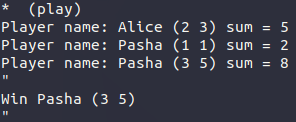
\includegraphics[width=0.5\textwidth]{img/5.png}
% 		\caption{Результат работы 5.} }
% \end{figure}

\newpage

\section*{Теоретическая часть}

\subsection*{Порядок работы и варианты использования функционалов}


\end{document}